\documentclass{beamer}
\usepackage[utf8]{inputenc}
\usepackage[T1]{fontenc}
\usepackage{lmodern}
\usepackage{amsmath}  % AMS mathematical facilities for LaTeX.
\usepackage{amsthm}   % Typesetting theorems (AMS style).
\usepackage{amsfonts} % 
\usepackage{mathrsfs}
\usepackage{amsmath,fourier}
\usepackage{amssymb}
\theoremstyle{remark}
\newtheorem{remark}{Remark}
\theoremstyle{plain}
\newtheorem{proposition}{Proposition}
\theoremstyle{plain}
\usetheme{Berlin} % Choose a theme (e.g., Madrid, Berlin, etc.)
\usecolortheme{default} % Choose a color theme (e.g., default, albatross, etc.)

% Customize the title page
\title[Spin-0 fields NP constants]{The cylinder at spatial infinity and asymptotic charges}
\author[Rafael Pinto]{Rafael Pinto}
\institute[CENTRA-GRIT]{Instituto Superior Técnico}
\date{\today}
% Add a logo to the title page (optional)
\titlegraphic{
\vspace{-15mm}
\includegraphics[width=1.5cm]{centra.png}
\hspace{\fill}

\includegraphics[width=1.5cm]{grit.png}
}

\begin{document}

% Title Page
\begin{frame}
  \titlepage
  \vfill
  \begin{center}
    Advisors: \textbf{Dr. Edgar Gasper\'in} and \textbf{Dr. Alex Va\~{n}\'o Vi\~{n}uales}
  \end{center}
\end{frame}

% Table of Contents (optional)
\begin{frame}{Table of Contents}
  \tableofcontents
\end{frame}

% Section 1: Introduction
\section{Newman-Penrose constants}
\begin{frame}{Introduction}
  \begin{itemize}
    \item The Newman-Penrose (NP) constants serve as conserved quantities at null infinity in asymptotically flat gravitational fields.
    \item These constants present a comprehensive conservation system for various spins: spin-1 fields and spin-2 fields, with our research focusing on spin-0 fields linked to wave equation solutions.
    \item In the detailed context, while an infinite series of conserved quantities is identified in the linear theory, the non-linear General Relativity theory conserves only ten.
  \end{itemize}
\end{frame}

\begin{frame}{Conservation laws}
  \begin{itemize}
    \item These charges are computed as 2-surface integrals at cuts ${C} \approx \mathbb{S}^2$ of null infinity $\mathscr{I}$.
  \end{itemize}
  \begin{figure}[h]
    \centering 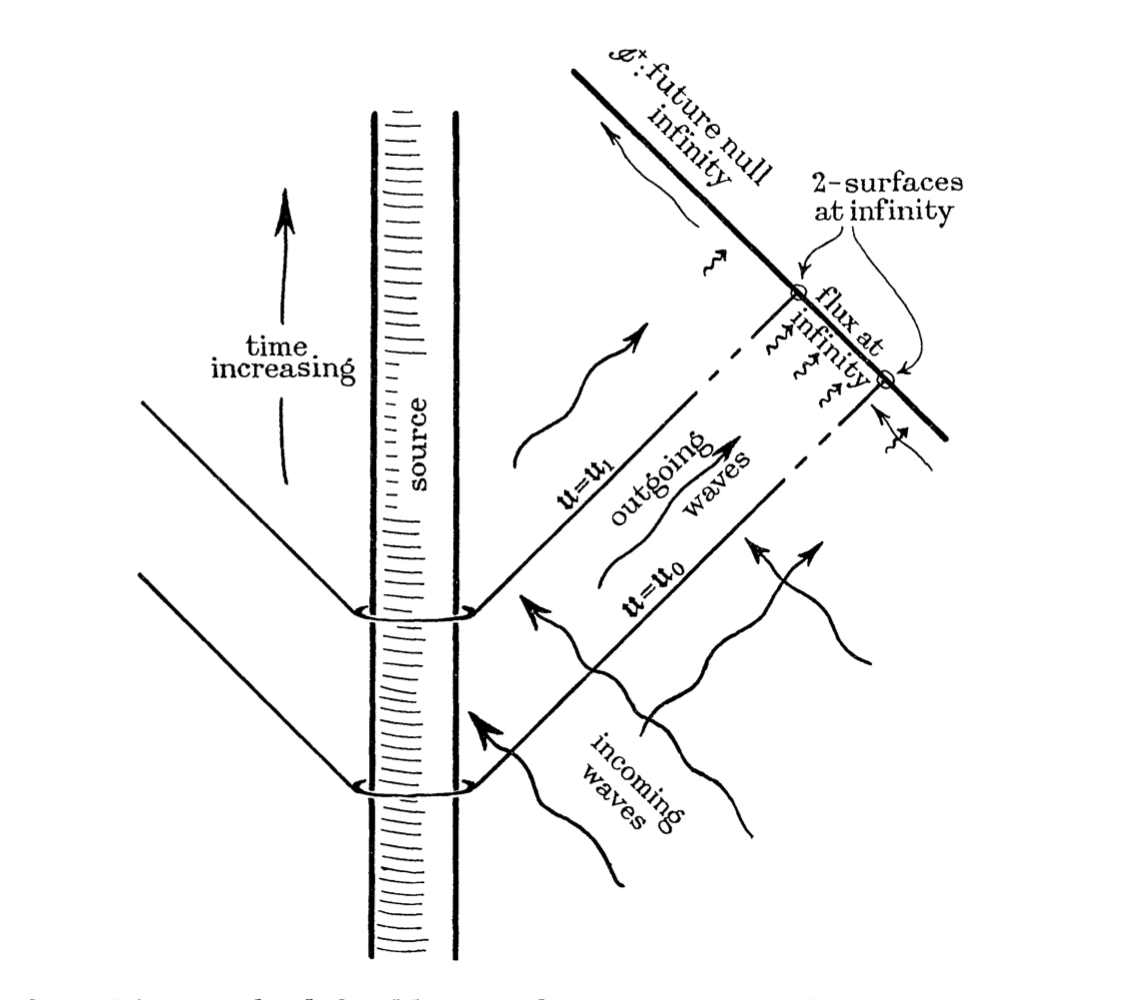
\includegraphics[width =0.45\textwidth]{penrose constants.png}
      \caption{Visual representation of the behavior of the Newman-Penrose constants at null infinity.}
  \end{figure}
\end{frame}

\begin{frame}{Spin-1 (EM) Field}
  \begin{itemize}
    \item A complex tetrad can be selected as follows:
      \begin{align}\label{eq:tetrad}
        & l^{\mu} = \delta_{1}^{\mu}, \quad n^{\mu} = \delta_{0}^{\mu} - \delta_{1}^{\mu}, \nonumber \\
        & m^{\mu} = \displaystyle\frac{1}{\tau}\left(\delta_{2}^{\mu} + \displaystyle\frac{1}{\sin\theta}\ \delta_{3}^{\mu}\right), \qquad \overline{m}^{\mu} = \displaystyle\frac{1}{\tau}\left(\delta_{2}^{\mu} - \displaystyle\frac{1}{\sin\theta}\ \delta_{3}^{\mu}\right).
      \end{align}
    \item To describe the electromagnetic (EM) field, we make use of three complex tetrad components of the Maxwell field tensor denoted as $F_{\mu \nu}$:
      \begin{align}\label{eq:Maxtensor}
        & \Phi_{0} = F_{\mu \nu}l^{\mu}n^{\nu}, \nonumber \\
        & \Phi_{1} = \frac{1}{2} F_{\mu \nu}(l^{\mu}n^{\nu} + \overline{m}^{\mu}m^{\nu}), \nonumber \\
        & \Phi_{2} = F_{\mu \nu}\overline{m}^{\mu}n^{\nu}.
      \end{align}
  \end{itemize}
\end{frame}

\begin{frame}{NP Constants Calculation}
  \begin{itemize}
    \item The NP constants are calculated using the following formula:
    \begin{equation}
      F_{m}^{n,k} = \int{_{1}\overline{Y}_{n-k+1,m}\Phi_{0}^{n+1} d\omega}.
    \end{equation}
    \item The interpretation of charges, such as the Newman-Penrose constants, remains an open debate, yet their conservation is evident in general asymptotically flat spacetimes, even in events like black hole collisions.
  \end{itemize}
\end{frame}
% Section 2: Literature Review
\section{Cylinder at $i^0$}
\begin{frame}{The $i^0$ cylinder representation in Minkowski  spacetime}
  % Your content for the literature review goes here
\end{frame}

% Section 3: Methodology
\section{Methodology}
\begin{frame}{Methodology}
  % Your content for the methodology goes here
\end{frame}

% Section 4: Results
\section{Results}
\begin{frame}{Results}
  % Your content for the results goes here
\end{frame}

% Section 5: Conclusion
\section{Conclusion}
\begin{frame}{Conclusion}
  % Your content for the conclusion goes here
\end{frame}

% References (optional)
\section{References}
\begin{frame}{References}
  % Your references go here
\end{frame}

% Thank You Slide
\begin{frame}{Thank You}
  % Thank your audience and any acknowledgments
\end{frame}

\end{document}
